\documentclass{beamer}

\usepackage{amsmath}
\usepackage{amssymb}
%\usepackage{textcomp}
\usepackage[ngerman]{babel}
\usepackage{caption}
\usepackage{dsfont}
\usepackage{graphicx}
\usepackage{color}
\usepackage{listings}
\usepackage{lmodern}
\usepackage[T1]{fontenc}
\usepackage[utf8x]{inputenc}

\graphicspath{{./imgs/}}

% customized theme
\usetheme{CambridgeUS}
\usecolortheme{whale}
\beamertemplatenavigationsymbolsempty
\setbeamertemplate{footline}[page number]
\setbeamercolor{frametitle}{fg=white,bg=structure}
\setbeamercolor{theorem}{fg=black,bg=structure!30}
\setbeamercovered{transparent}

\definecolor{mygreen}{rgb}{0, 0.6, 0}
\definecolor{mymauve}{rgb}{0.58, 0, 0.82}

\lstset{
	language=Python,
	breaklines=true,
	tabsize=4,
	%basicstyle=\ttfamily,
	keywordstyle=\color{blue},
	stringstyle=\color{mymauve},
	commentstyle=\color{mygreen},
	otherkeywords={
		None,False,True,
		self,
		bytes}
}

% meta informations for title page
\title{Abschlusspräsentation}
\subtitle{Visual Analytics für raumzeitliche Daten}
\author{Christian Diehr \and Benjamin Drost \and David Foerster}
\institute{Institut für Informatik\\Humboldt-Universität zu Berlin}
\logo{
\includegraphics[width=2cm,height=2cm]{imgs/hulogo.pdf}}
\date{16. Februar 2016}

\begin{document}

    \begin{frame}
        \titlepage
    \end{frame}
    \logo % logo only appears on title page

    \section{Clustering}
	% Erklären, was Clustering ist
	% Erklären, wie der kMeans-Algorithmus funktioniert
	% KMeans einfach, häufig verwendet
	% Abhängigkeit von gewähltem Startpunkt als Nachteil
    \begin{frame}{k-Means-Algorithmus}
		\begin{figure}
			\centering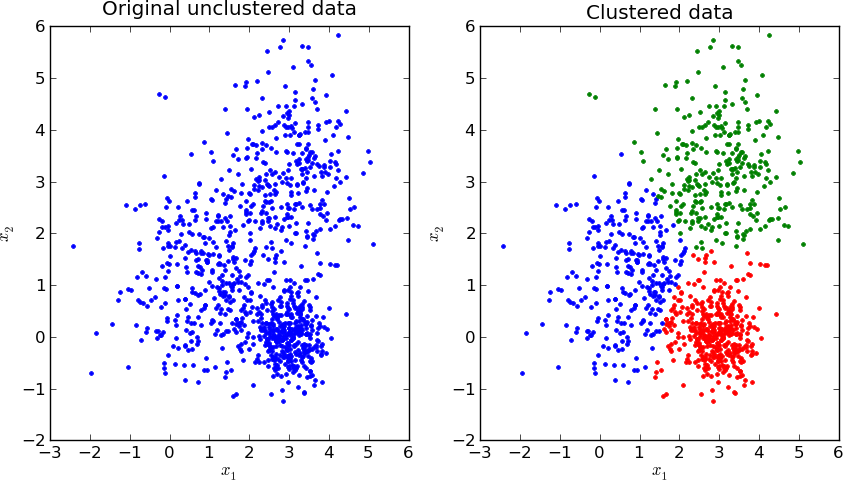
\includegraphics[width=.7\textwidth]{kmeans.png}
			\setbeamertemplate{caption}{\raggedright\insertcaption\par}
			\caption{Quelle: pypr.sourceforge.net/\_images}
			\setbeamertemplate{caption}[default]
		\end{figure}
    \end{frame}

    \begin{frame}{Datenpunkte im $\mathds{R}^{31}$}
    	\begin{figure}
    		\centering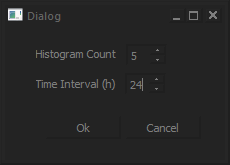
\includegraphics[width=.4\textwidth]{dialog.png}
    	\end{figure}
    	\begin{itemize}
    		\setlength\itemsep{1em}
    		\item Aggregation über Intervalllänge
    		\item Anzahl Histogramme $\simeq$ Anzahl Zentroide
    	\end{itemize}
    \end{frame}

    \begin{frame}{Beispiel eines Clusterings}
    	% Farben nach Anzahl der kleinsten Korngröße sortiert
    	% dunkle Farben = höchste Staubkonzentration
    	\begin{figure}
    		\centering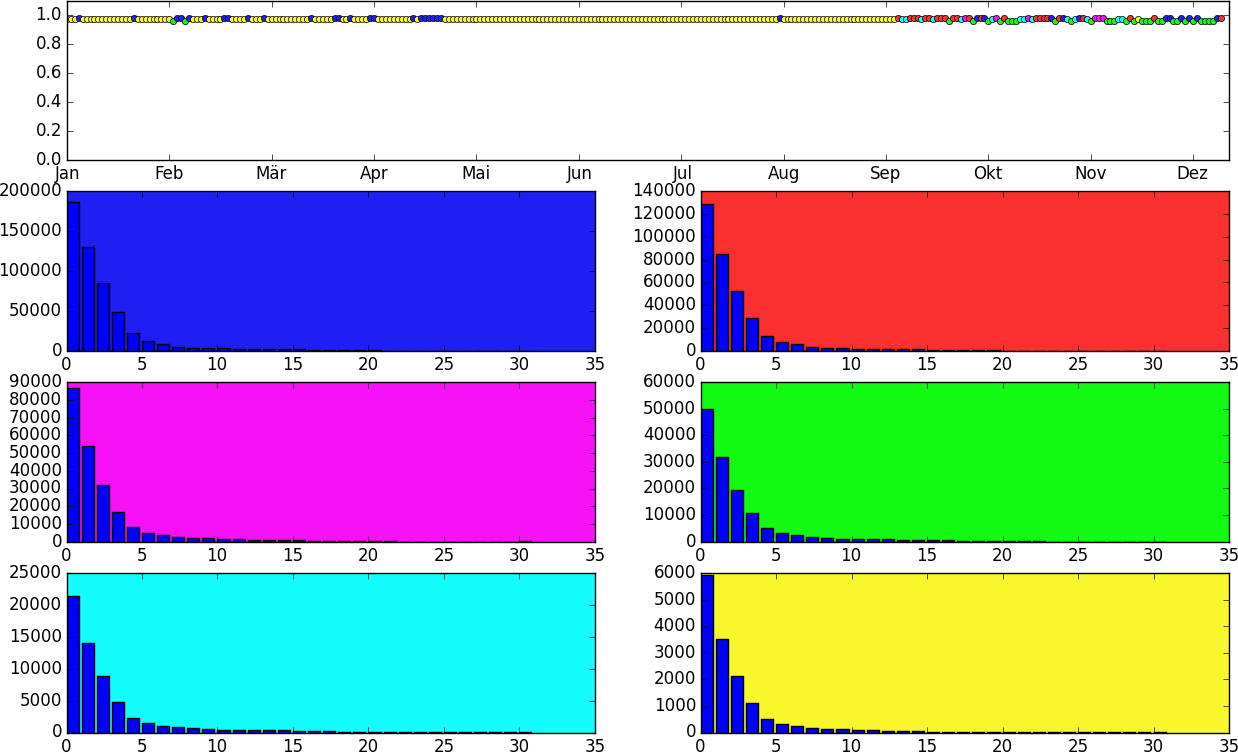
\includegraphics[width=\textwidth]{histogramm.png}
    	\end{figure}
    \end{frame}

    % Live-Demonstration des Clusterings

    \section{Ziele}
    \begin{frame}{Ziel 1}
    	% Frage leicht anders interpretiert ohne den Zusatz des bestimmten Zeitintervalls
    	\begin{itemize}
    		\setlength\itemsep{1em}
    		\item[] \textit{Welche unterschiedlichen Typen von Verteilungen gibt es in einem bestimmten Zeitintervall?}
    		\item[]
    		\item alle Verteilungen über das gesamte Jahr entsprechen einer umgekehrten Proportionalität
    		\item umgekehrte Proportionalität $\sim k/g$, mit $k$ einem Zentroidfaktor und $g$ der Korngröße
    	\end{itemize}
    \end{frame}

    \begin{frame}{Ziel 2}
    	\begin{itemize}
    		\setlength\itemsep{1em}
    		\item[] \textit{Wann treten diese Typen in diesem Zeitintervall auf?}
    		\item[]
    		\item von Januar bis einschließlich August ein Typ, Abweichungen Anfang Februar für 5 Tage und Mitte April für 7 Tage
    		\item ab September höhere Staubkonzentrationen (vermutlich durch Niederschlag)
    	\end{itemize}
    \end{frame}

    \begin{frame}{Ziel 3}
    	\begin{itemize}
    		\setlength\itemsep{1em}
    		\item[] \textit{Wann verändern sich sich die Typen, wenn der Anwender das Zeitfenster verändert?}
    		\item[]
    		\item Typen verändern sich für 12h, 24h, 36h, 48h und 72h kaum, Plot wird nur gröber
    	\end{itemize}
    \end{frame}

    \begin{frame}{Vorteile}
    	\begin{itemize}
    		\setlength\itemsep{1em}
    		\item[] \textit{Demo von 3 Vorteilen für die Exploration der Staubdaten}
    		\item[]
    		\item
    	\end{itemize}
    \end{frame}

%    \section{Histogramm}
%    \begin{frame}{Histogramm-Optionen}
%		\begin{itemize}
%			\setlength\itemsep{1em}
%			\item Im Histogramm-Dialog Einstellungen auswählen
%			\begin{itemize}
%				\setlength\itemsep{1em}
%				\item Intervallgröße festlegen
%				\item Monat wählen
%				\item Darzustellende Partikel bestimmen
%			\end{itemize}
%			\item Darstellung per matplotlib
%			\item Tooltip erscheint bei Berührung einer Bar im Histogramm
%		\end{itemize}
%    \end{frame}

\end{document}
